% 英文引号
\newcommand{\enquote}[1]{``{#1}''}
% 中文引号
\newcommand{\zhquote}[1]{“{#1}”}
% 方框
\renewcommand{\Box}{\mdlgwhtsquare}
% 对勾
\newcommand{\checkbox}{$\checkmark$}
% 勾选了对勾的方框
\newcommand{\checkedbox}{\mbox{\mdlgwhtsquare\hspace{-0.75em}\raisebox{0.15ex}{$\checkmark$}}}
% 学位类型View
\newcommand{\degreetype}{ % 学位类型
  \ifthenelse{\equal{\isacademicdegree}{true}}
  {
    {\fangsong\zihao{3} \checkedbox 学术学位\hspace{2em} \zihao{3} \Box 专业学位}
  }
  {
    {\fangsong\zihao{3} \Box 学术学位\hspace{2em} \zihao{3} \checkedbox 专业学位}
  }
}
% Copyright (c) 2008-2009 solvethis
% Copyright (c) 2010-2017,2021 Casper Ti. Vector
% Copyright (c) 2021 Kurapica
% Copyright (c) 2021 iofu728
% All rights reserved.
%
% Redistribution and use in source and binary forms, with or without
% modification, are permitted provided that the following conditions are
% met:
%
% * Redistributions of source code must retain the above copyright notice,
%   this list of conditions and the following disclaimer.
% * Redistributions in binary form must reproduce the above copyright
%   notice, this list of conditions and the following disclaimer in the
%   documentation and/or other materials provided with the distribution.
% * Neither the name of Peking University nor the names of its contributors
%   may be used to endorse or promote products derived from this software
%   without specific prior written permission.
%
% THIS SOFTWARE IS PROVIDED BY THE COPYRIGHT HOLDERS AND CONTRIBUTORS "AS
% IS" AND ANY EXPRESS OR IMPLIED WARRANTIES, INCLUDING, BUT NOT LIMITED TO,
% THE IMPLIED WARRANTIES OF MERCHANTABILITY AND FITNESS FOR A PARTICULAR
% PURPOSE ARE DISCLAIMED. IN NO EVENT SHALL THE COPYRIGHT HOLDER OR
% CONTRIBUTORS BE LIABLE FOR ANY DIRECT, INDIRECT, INCIDENTAL, SPECIAL,
% EXEMPLARY, OR CONSEQUENTIAL DAMAGES (INCLUDING, BUT NOT LIMITED TO,
% PROCUREMENT OF SUBSTITUTE GOODS OR SERVICES; LOSS OF USE, DATA, OR
% PROFITS; OR BUSINESS INTERRUPTION) HOWEVER CAUSED AND ON ANY THEORY OF
% LIABILITY, WHETHER IN CONTRACT, STRICT LIABILITY, OR TORT (INCLUDING
% NEGLIGENCE OR OTHERWISE) ARISING IN ANY WAY OUT OF THE USE OF THIS
% SOFTWARE, EVEN IF ADVISED OF THE POSSIBILITY OF SUCH DAMAGE.
\newcommand{\origin}
{
	\ctexset{section = {
		format+ = {\centering}, beforeskip = {40bp}, afterskip = {15bp}
	}}
	\specialchap{北京大学学位论文原创性声明和使用授权说明}

	% 学校书面要求本页面不要页码,但在给出的 Word 模版中又有页码。
	% 此处以学校书面要求为准。
	\thispagestyle{empty}
	
	% 替换扫描pdf,去除includegraphics前注释
	\begin{textblock}{1}(-0.8,-0.08)
		\colorbox{white}{
			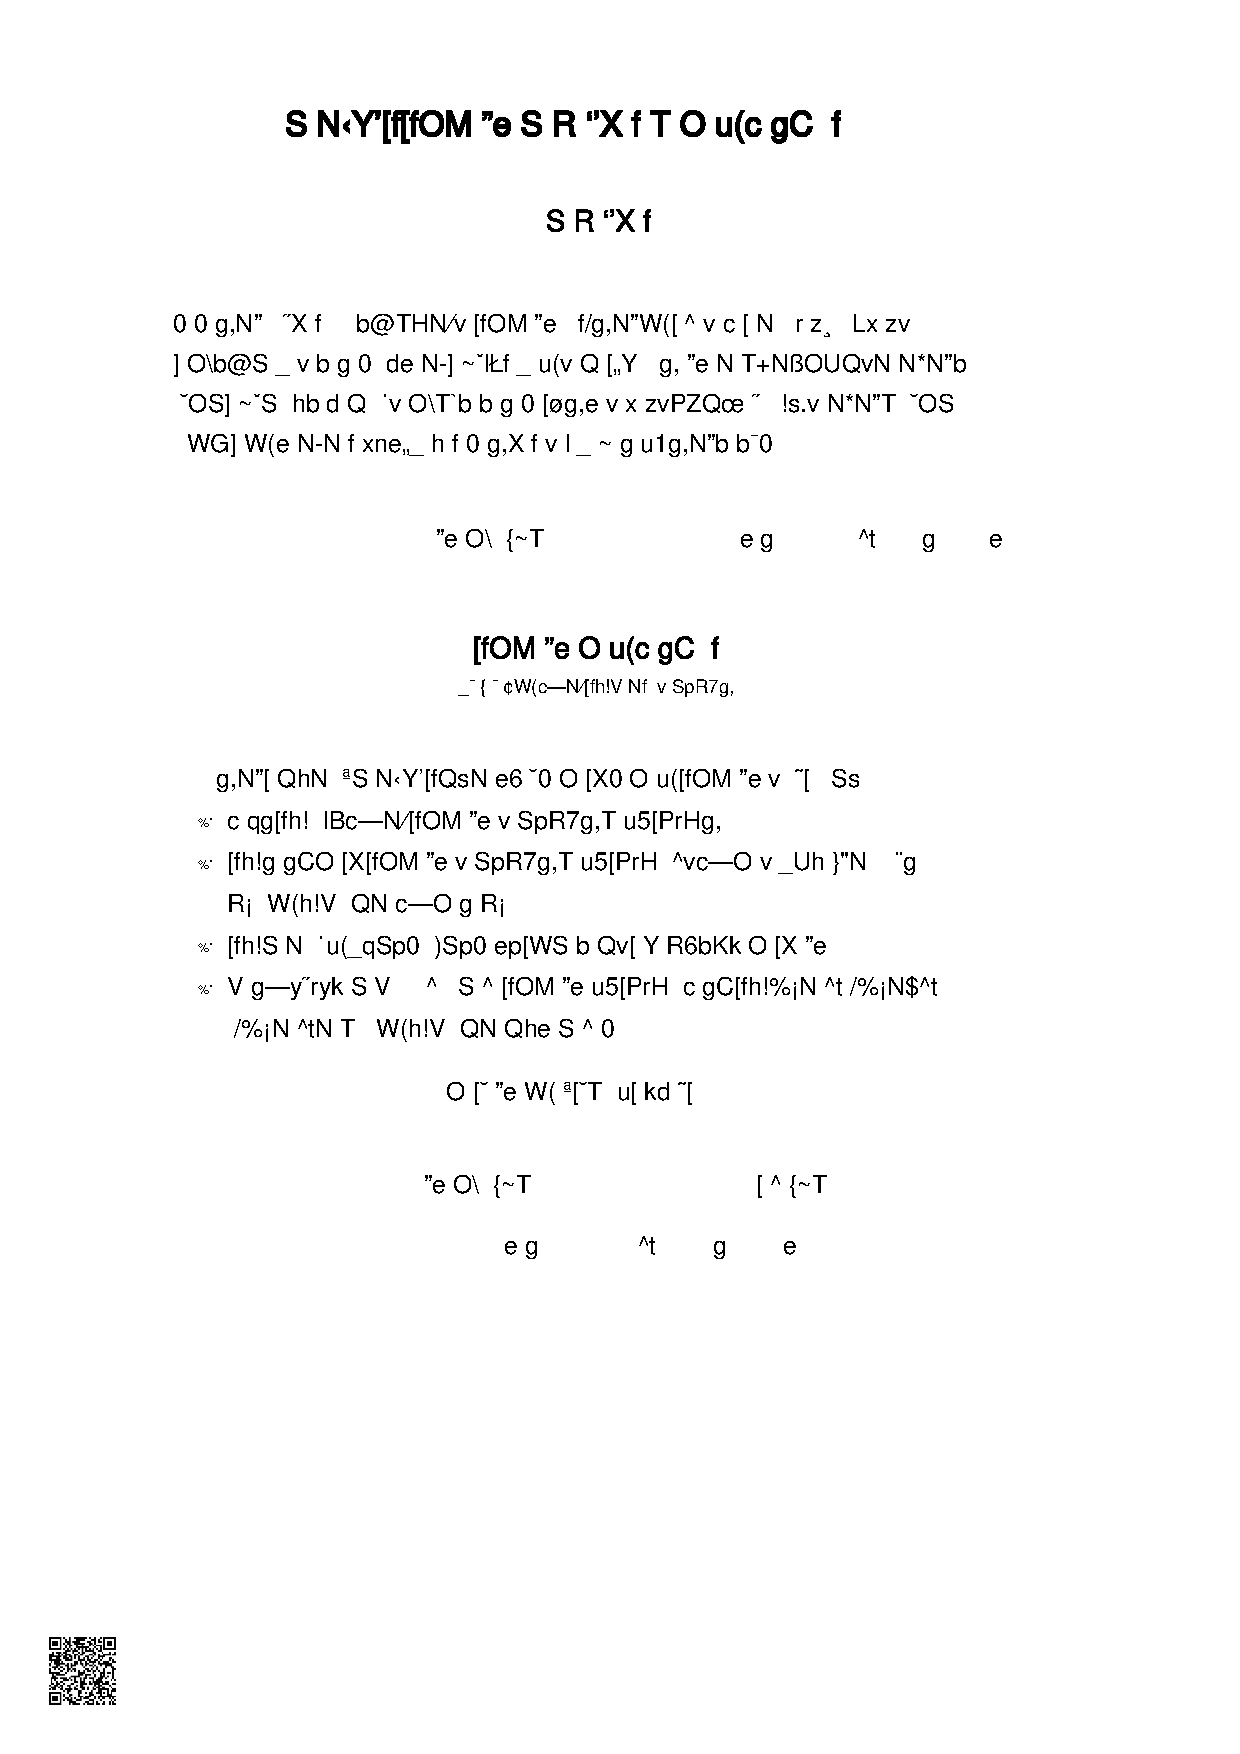
\includegraphics[height = 1.2448\textheight]{原创性声明.pdf}
		}
	\end{textblock}
}

% vim:ts=4:sw=4

\pkuthssinfo{
    cthesisname = {硕士学位论文},
    thesiscover = {硕士研究生学位论文},
    ethesisname = {Master Thesis},
    ctitle = {\zhtitle},
    etitle = {\entitle},
    cauthor = {\zhauthor}, eauthor = {\enauthor},
    studentid = {\thestudentid},
    % 具体时间以教务为准,初稿3月,送审4月,答辩5月,最终6月。
    date = {\zhdigits{\theyear}\ \ 年\ \ \zhnumber{\themonth}\ \ 月}, % June, 2022
    school = {汇丰商学院},
    cmajor = {\zhmajor}, emajor = {\enmajor},
    direction = {\majordirection},
    % 副教授 A.P. 讲师 Lec.
    cmentor = {\zhmentor}, ementor = {\enmentor},
    ckeywords = {\zhkeywords}, ekeywords = {\enkeywords},
    % 盲审模式参数, 需在documentclass增加blind
    % blindid = {XXXXXXXXX}, discipline = {XXXX}
}
